% CI head f028ec5 / tested merge ae11d8b: RTL job succeeds; workflow conclusion remains separate.
% Both preceding local 169f and failed-job 0c4a generated artifacts are retained under history/.
\clearpage
\section{成功 RTL job 的 21 项图证与独立算术验收}
\label{sec:historical-21-evidence}
\label{sec:ci-21-evidence}
本节四幅图改用 \code{docs/evidence/20260930/ci_rtl_f028/} 的真实 CI 日志。
\textbf{21 项 RTL bench、3 类严格 lint 和独立算术审计均通过，本次 RTL job 的结论为 success。}
归档抓取时 workflow 仍为 \code{in_progress}，不能由一个 job 成功推断整个 workflow 全绿。
归档 head 为 \code{f028ec5}，实际测试 merge 为 \code{ae11d8b}，两者完整 Git tree 均为 \code{d84022bd}…；生产 RTL 内容摘要为 \code{fd885e882ad5}…。
这是已发布精简版的验收记录，不能提前归给正在开发的缓存等新候选结构；候选结构须以其独立源码摘要和实跑结果另行验收。
制图器核验归档清单、日志、步骤结论以及 head 中 87 项输入的实际字节，不用当前工作树替代历史输入。
样本、输入码、断言和检查节拍分别保留单位，不相加为覆盖率。

\begin{figure}[H]\centering
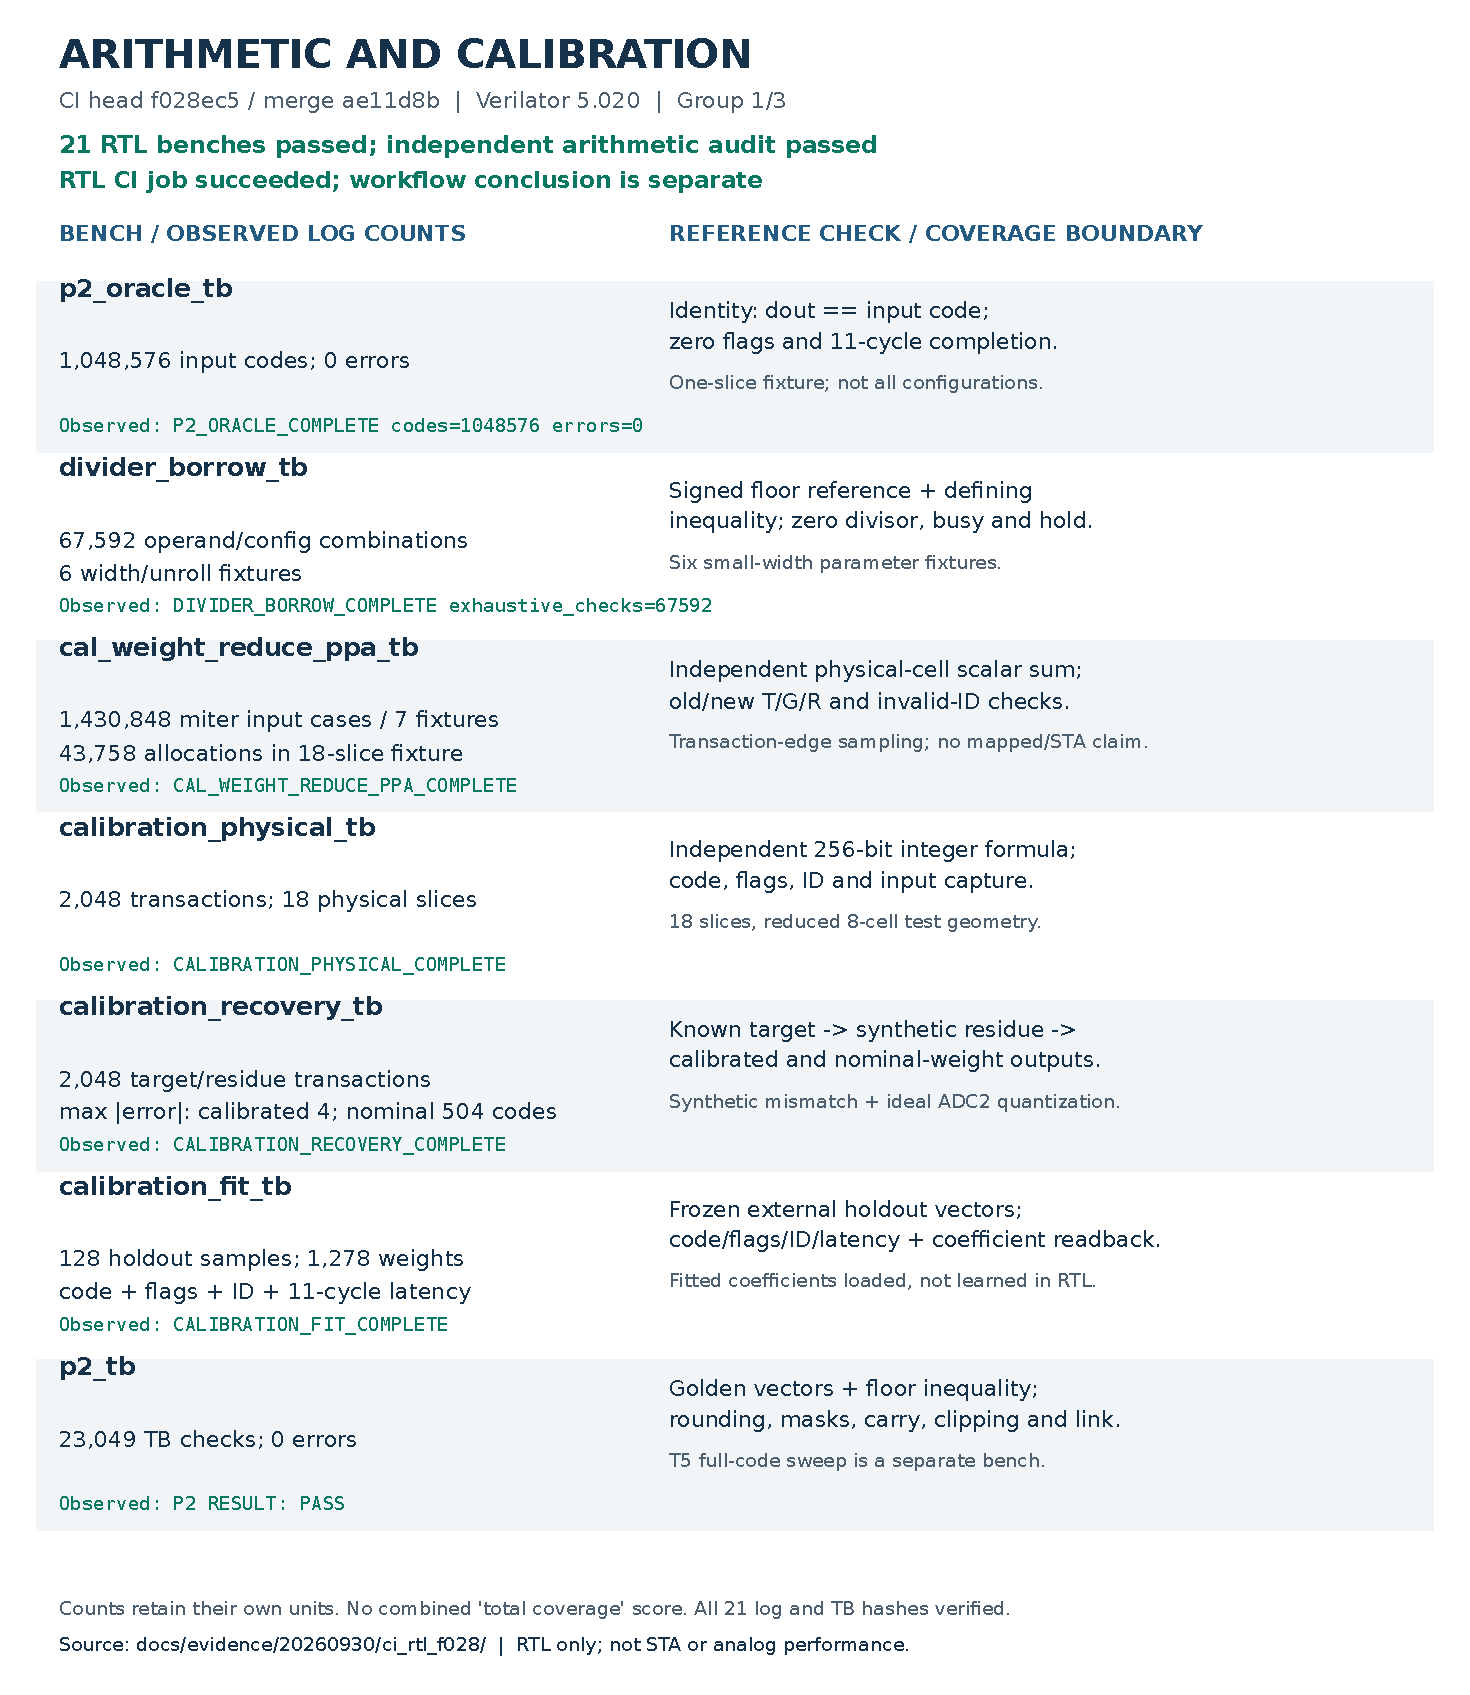
\includegraphics[width=.96\textwidth]{figures/final_regression_arithmetic.pdf}
\caption{本次 CI 中算术与校准的七项 RTL 回归。归约器同时比较新旧结果与独立物理单元 scalar 求和；另行执行并通过的独立算术审计在本节后部说明。全码恒等和除法穷举分别受简化配置及六组小位宽的范围限制。}
\label{fig:final-regression-arithmetic}
\end{figure}

\clearpage
\subsection{事务、取消与结构调度}
图\ref{fig:final-regression-protocol}中的结构顶层运行使用 P7，438 次输出逐笔对应 438 次延迟检查，7,680 是协议检查节拍数。
独立 \code{recon_ppa_latency_tb} 在这次 CI 中也重新执行 P5/P6/P7 各 32 笔连续启动，间隔 16 拍，延迟 15/13/11 拍，busy 释放 14/12/10 拍。
这是新 CI 的结果，不是将旧 \code{final_profiles/} 日志改名。
\code{review_recon_protocol_tb} 未打印总计数；\code{review_top_protocol_tb} 的 38 仍按测试台打印值标注。

\begin{figure}[H]\centering
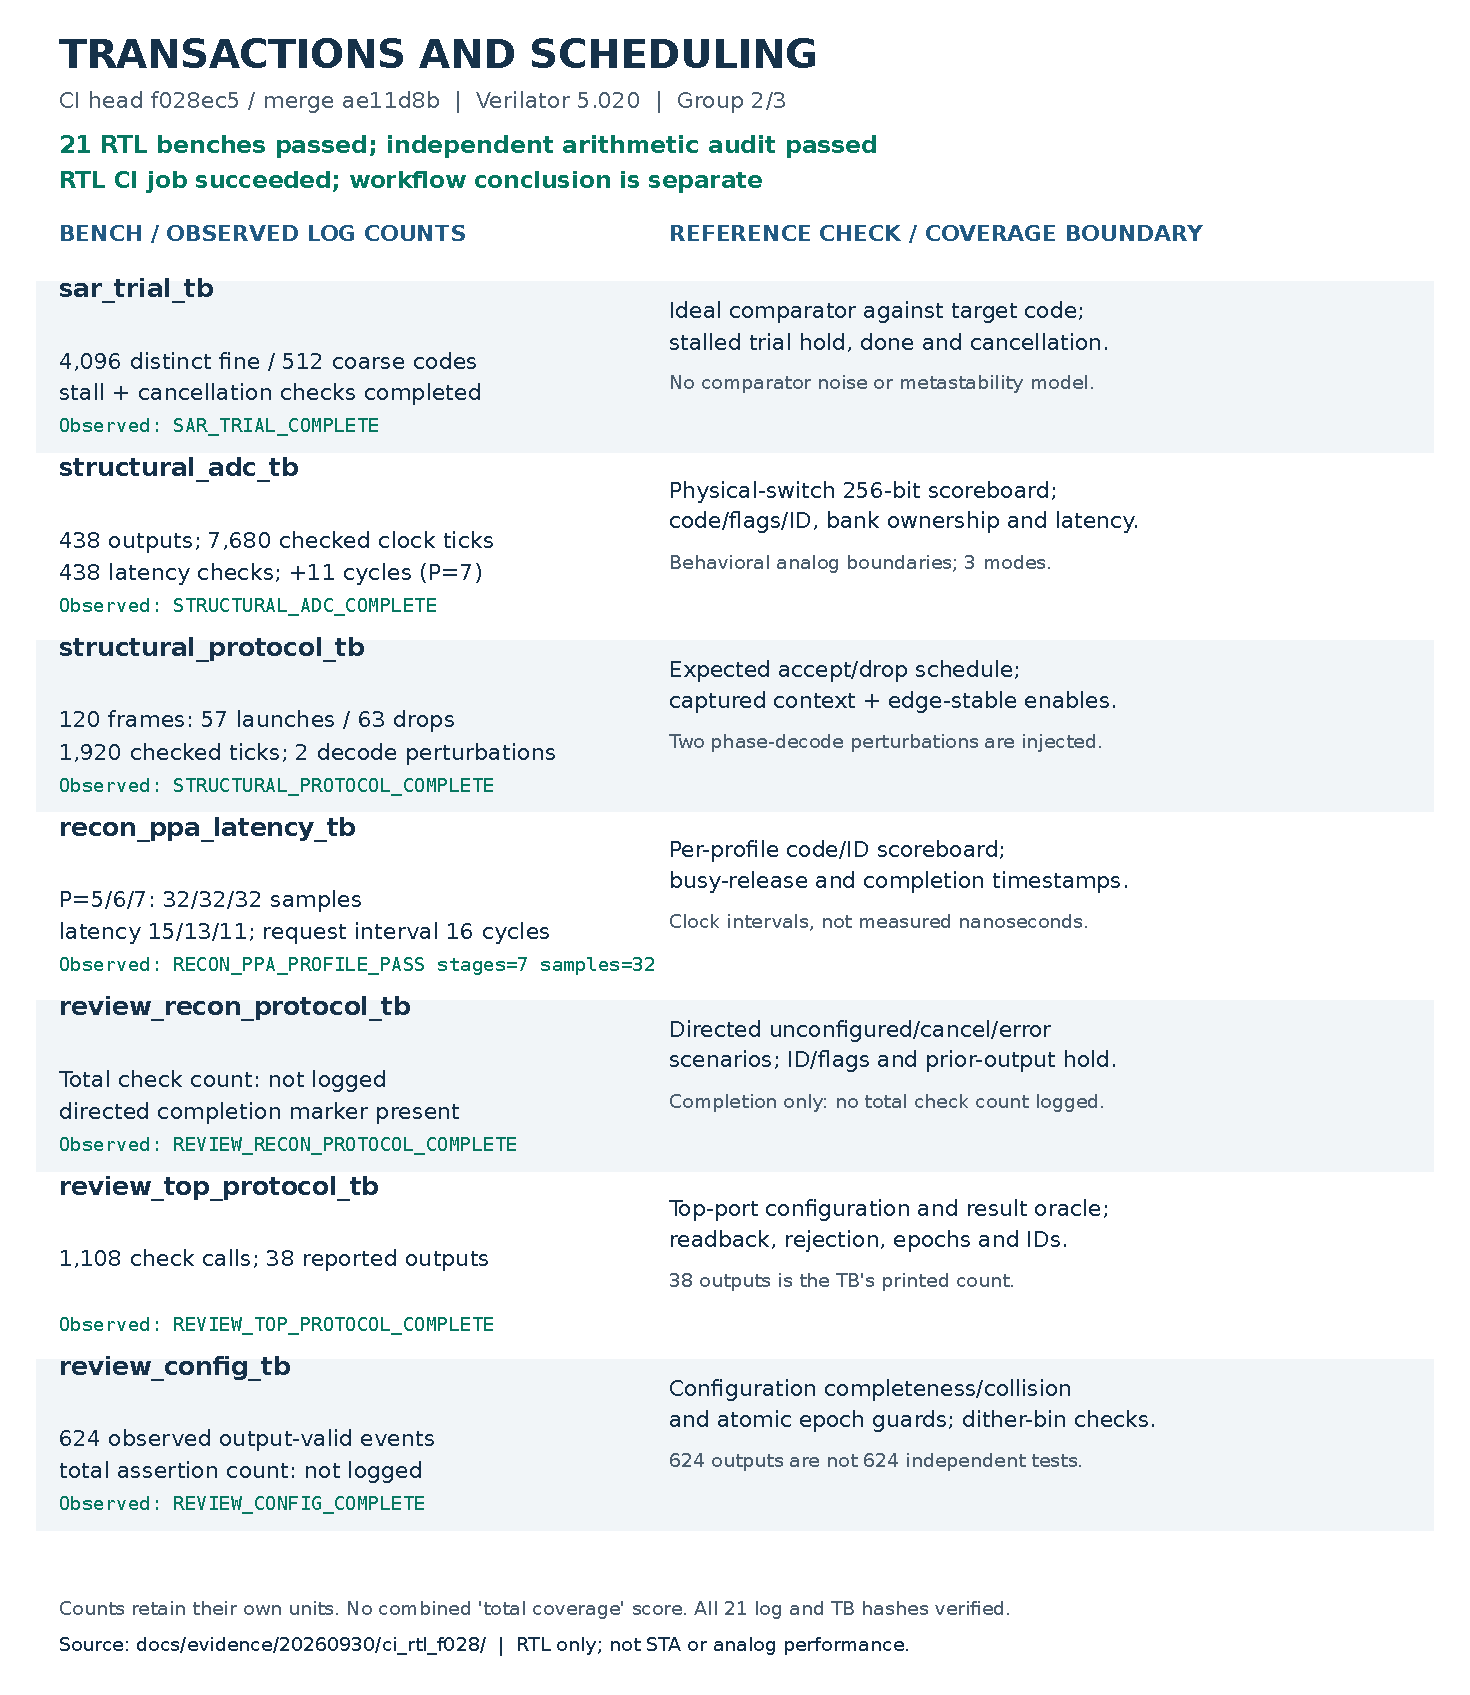
\includegraphics[width=\textwidth]{figures/final_regression_protocol.pdf}
\caption{本次 CI 的七项事务与调度证据，覆盖 SAR 停顿/取消、上下文隔离、ID/flags 对齐、配置屏蔽和 epoch 取消。图中为功能时钟间隔，不是门级纳秒延迟或 640\,MHz 时序签核。}
\label{fig:final-regression-protocol}
\end{figure}

\clearpage
\subsection{基础模块、配置和兼容顶层}
图\ref{fig:final-regression-system}保留每个测试原有计数器的含义。
外设各小计是累计值；dither 的七种条件分别在 200,000 个观测周期内接收 196,866 或 200,000 笔输出。
\code{tree_mapping_tb} 在此次 CI 中是 Verilator RTL 运行，不能改称真实网表仿真。

\begin{figure}[H]\centering
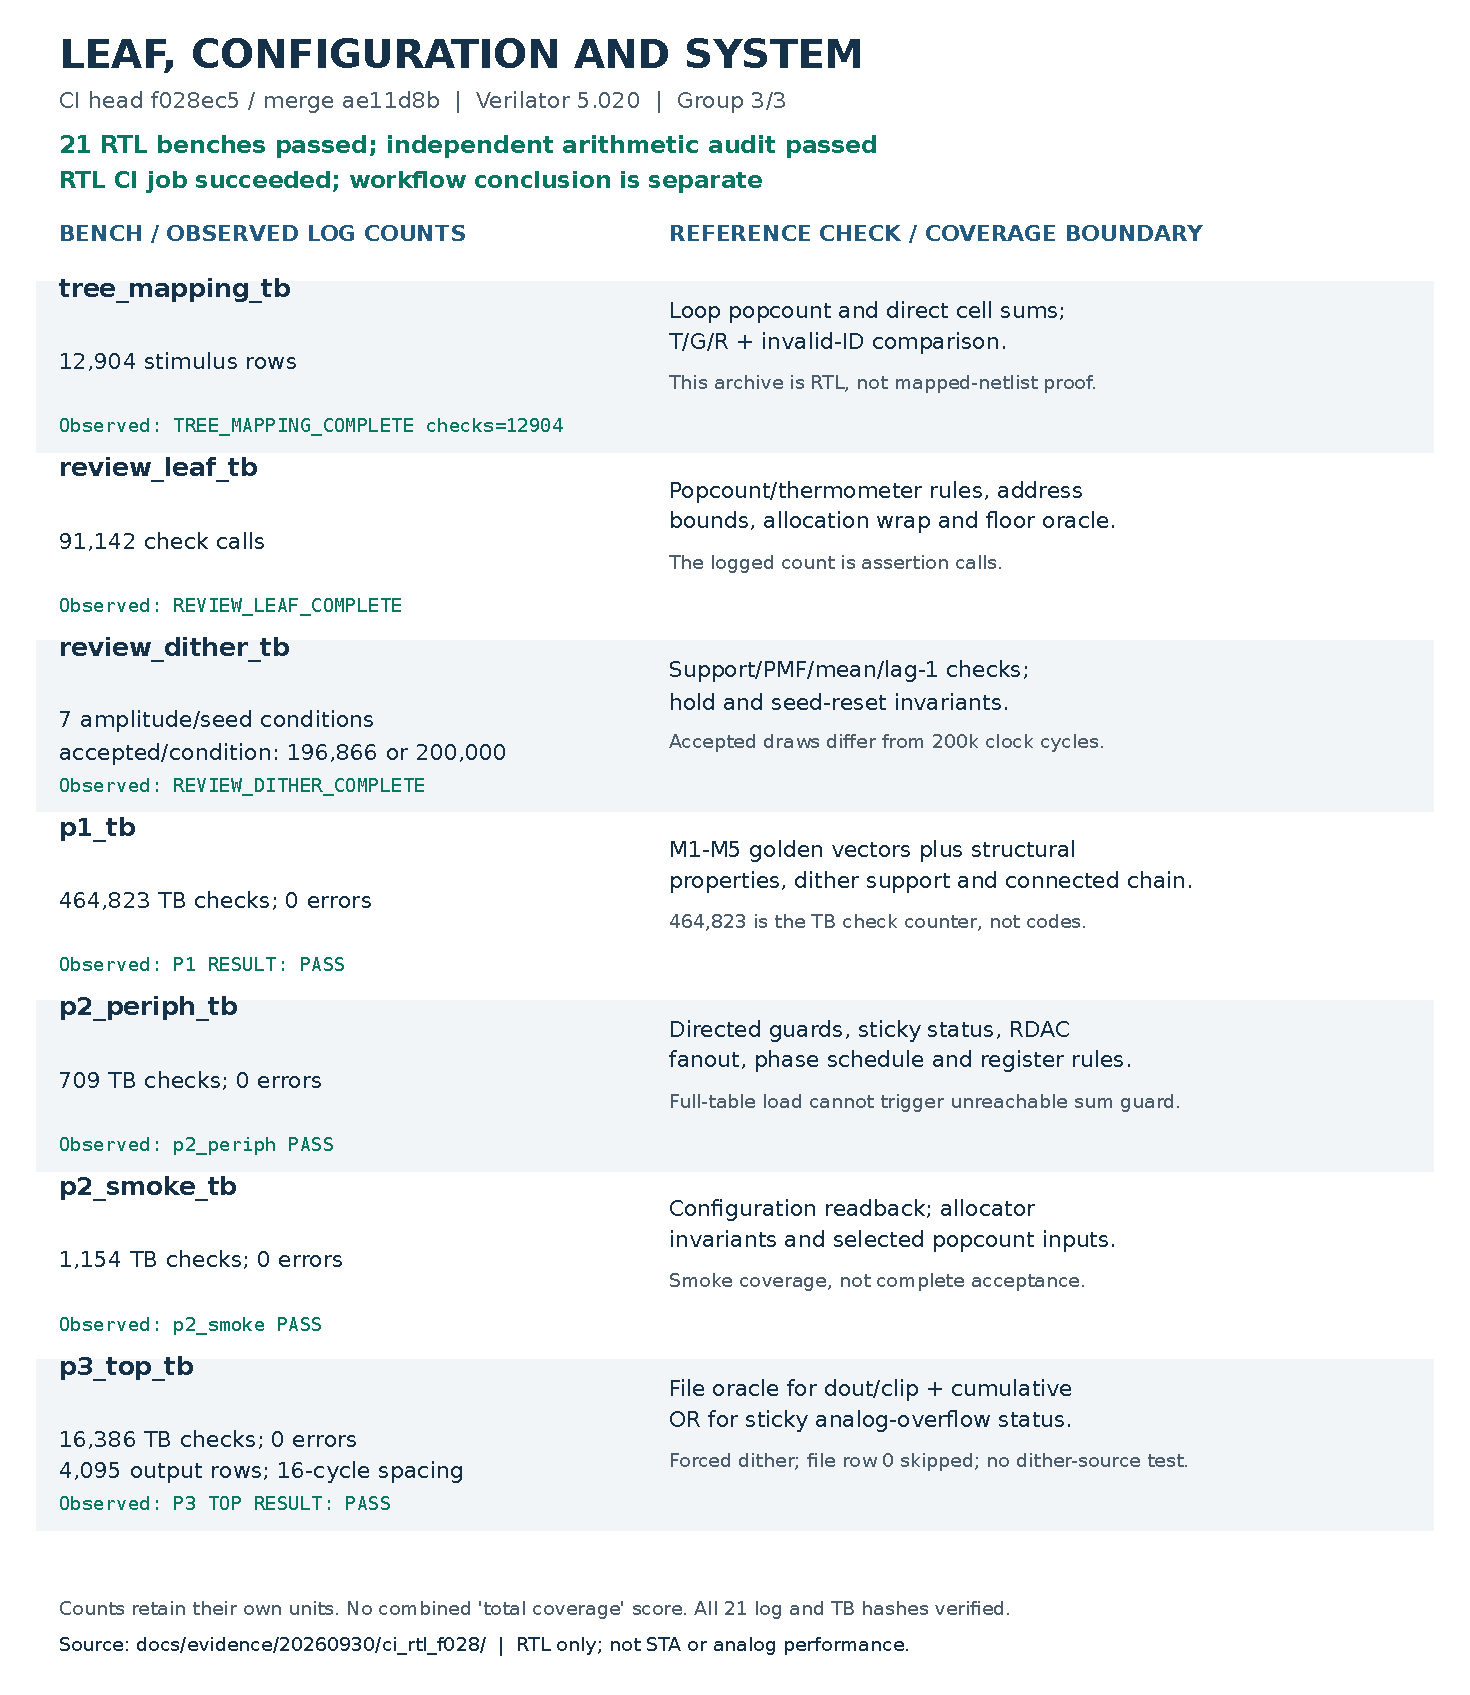
\includegraphics[width=\textwidth]{figures/final_regression_system.pdf}
\caption{本次 CI 中基础模块、配置与兼容顶层的七项证据。兼容顶层比较 4,095 行输出，跳过向量第 0 行，并 force 注入 dither；因此不覆盖该模式下片内 dither 源。analog-overflow 仍按累计 OR 的粘滞语义比较。}
\label{fig:final-regression-system}
\end{figure}

\clearpage
\subsection{新日志中的定量观测}
图\ref{fig:final-regression-quantitative}的 A、B 面板读取本次 CI 全部 128 条 \code{FIT_ROW}：码值、flags、ID 均相符，延迟均为 11 拍。
横轴是留出样本序号；这些数据来自外部拟合系数的加载和重构，并不是片上参数学习或模拟瞬态测量。
C 面板只有日志记录的两项最大绝对误差：标称权重 504 码、校正权重 4 码，不由两根柱子推导 RMS、SNDR 或 ENOB。

\begin{figure}[H]\centering
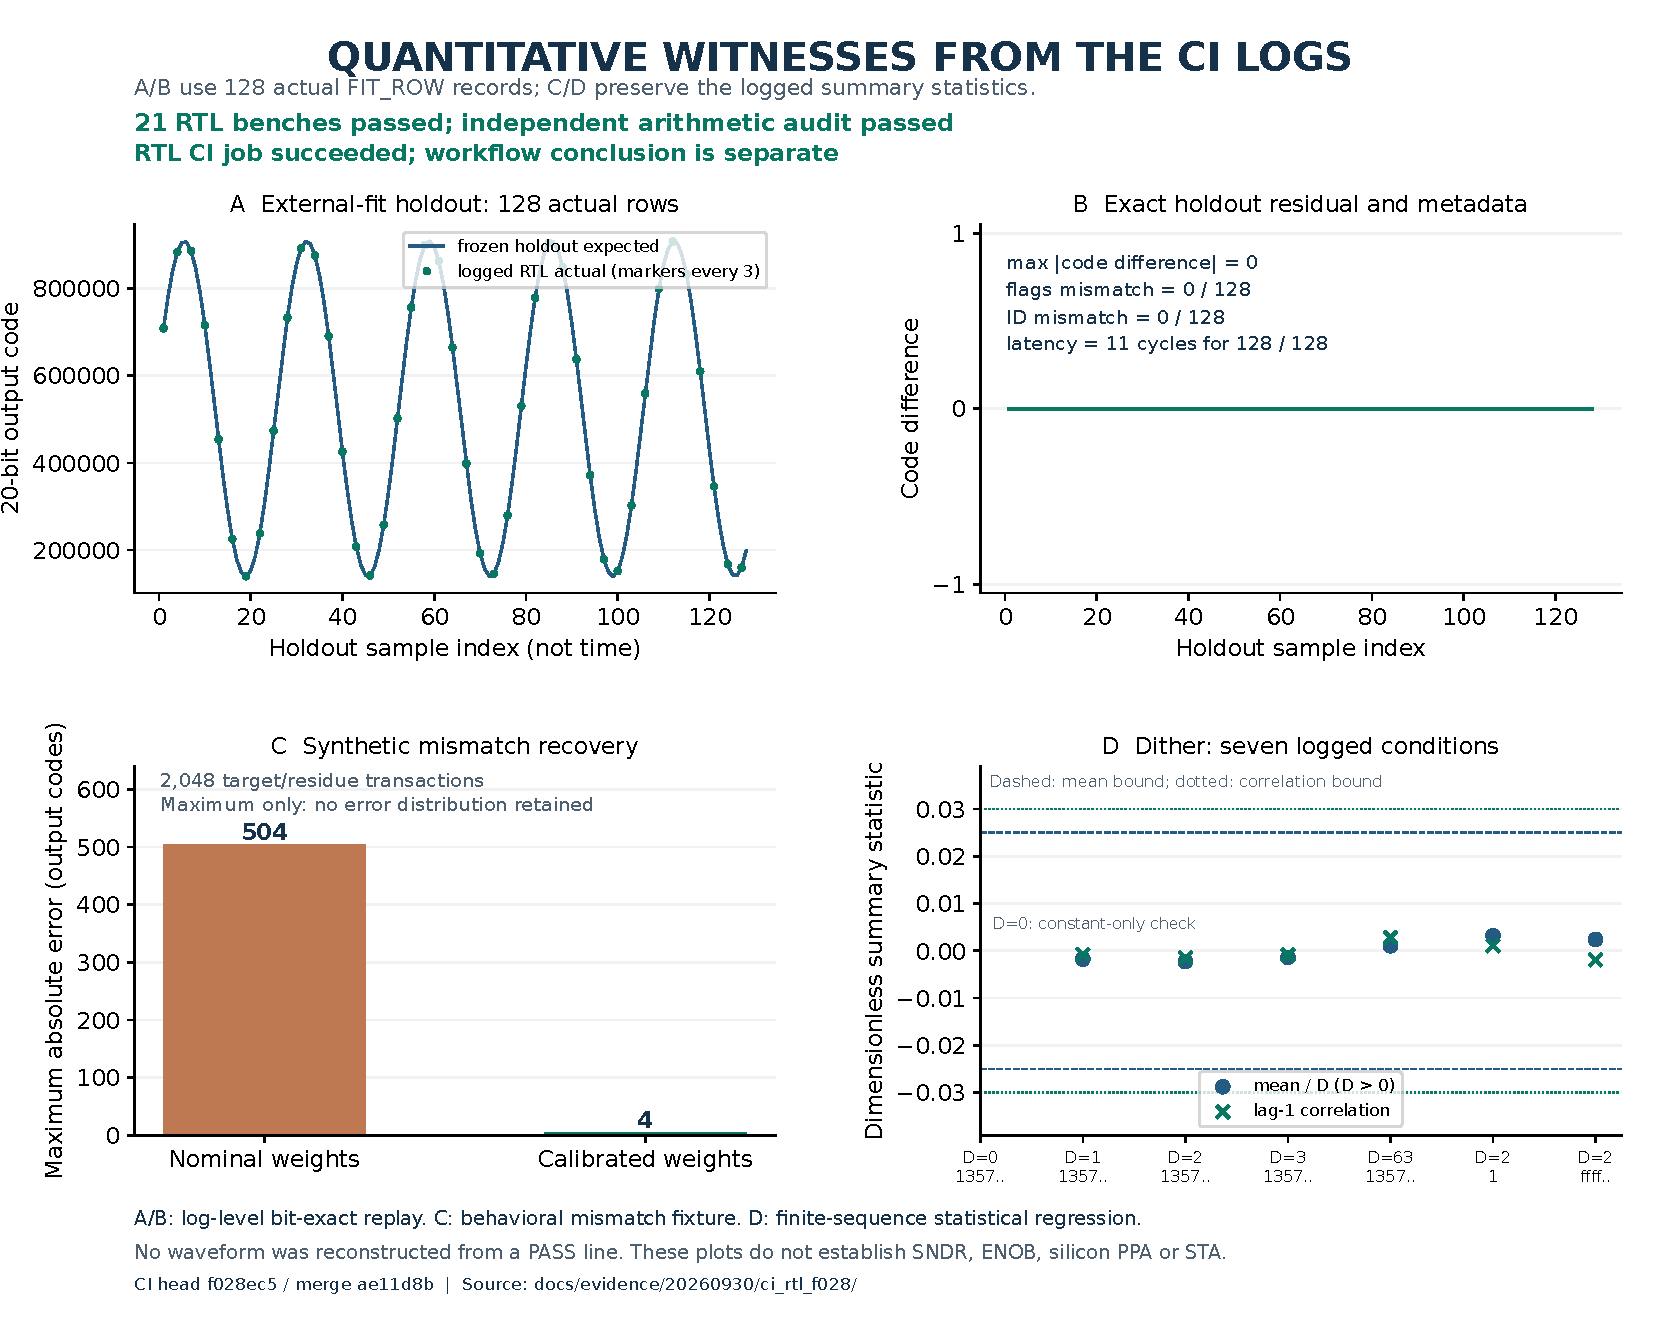
\includegraphics[width=\textwidth]{figures/final_regression_quantitative.pdf}
\caption{本次 CI 日志的实际数值。A/B 为 128 笔留出数据；C 为 2,048 笔合成失配的最大误差摘要；D 为七组 dither 的打印统计量，均值除以幅度 $D$，门限分别为 $\pm0.025$ 与 $\pm0.03$。$D=0$ 方差为零，相关性不计算，也不画成有效零值。}
\label{fig:final-regression-quantitative}
\end{figure}

D 面板均值/相关性只保留日志的六位小数。原日志没有各 PMF bin，因此不能补画分布；其余三图使用证据矩阵，不从完成标记伪造波形。
归约器参考计算和判据位于该 head 的 \code{sim/tb/cal_weight_reduce_ppa_tb.sv:47} 至 109 行：独立 scalar 函数读取原始刺激，同时验证两份实现的 \(T,G,R\) 与非法地址标志。
本次 5.020 CI 完成七种几何、1,430,848 次检查；43,758 个生产分配组合包含在这些检查中。
另外的本地双版本复验与共同错误负控仍按图\ref{fig:reducer-scheduler-evidence}的原来源保留。

\subsection{独立算术审计：CI 成功与本地双版本负控}
历史 \code{0c4a772} CI 的独立审计未进入仿真：runner 将头文件安装目录设置为 \code{VERILATOR_ROOT}，使已安装启动器寻找不存在的 \code{verilator_bin}，以 127 返回。
该失败仍保留于旧 \code{ci_rtl_0c4a/arithmetic_entry_failure.log}；不得因后续修复而覆盖其失败状态。

\begingroup\raggedright
随后修复启动路径，并处理本机 5.020 暴露的文件刺激调度问题，形成独立归档 \code{docs/evidence/20260930/arithmetic_runner_ci/}。
两种记录的工具版本分别完整通过 40,010 项 MAC（其中 20,859 项不溢出）、40,000 项 ADC2、10,048 笔除法和 8 组 flags 序列。
保持陈旧 MAC 输入和固定 ADC 输入的两个负控分别在 MAC 第 3 行、ADC 第 2 行失败；另有 8 项路径/环境单测通过。
这些本地结果保持生产 RTL 和期望向量不变，但修复了审计 runner 和 TB，不能倒写为 \code{0c4a772} 的独立审计通过。
本次 \code{f028ec5} 在 Ubuntu/Verilator 5.020 上随后也完成同样的独立审计，
真实日志与 manifest 位于 \code{ci_rtl_f028/arithmetic-audit/}，七项受检源文件与被测 Git tree 一致。
这使本次 RTL job 完整成功；其余 workflow jobs 的最终结论另由 \code{ci_workflow_f028/} 记录为9项全部成功。\par\endgroup

\begin{figure}[htbp]\centering
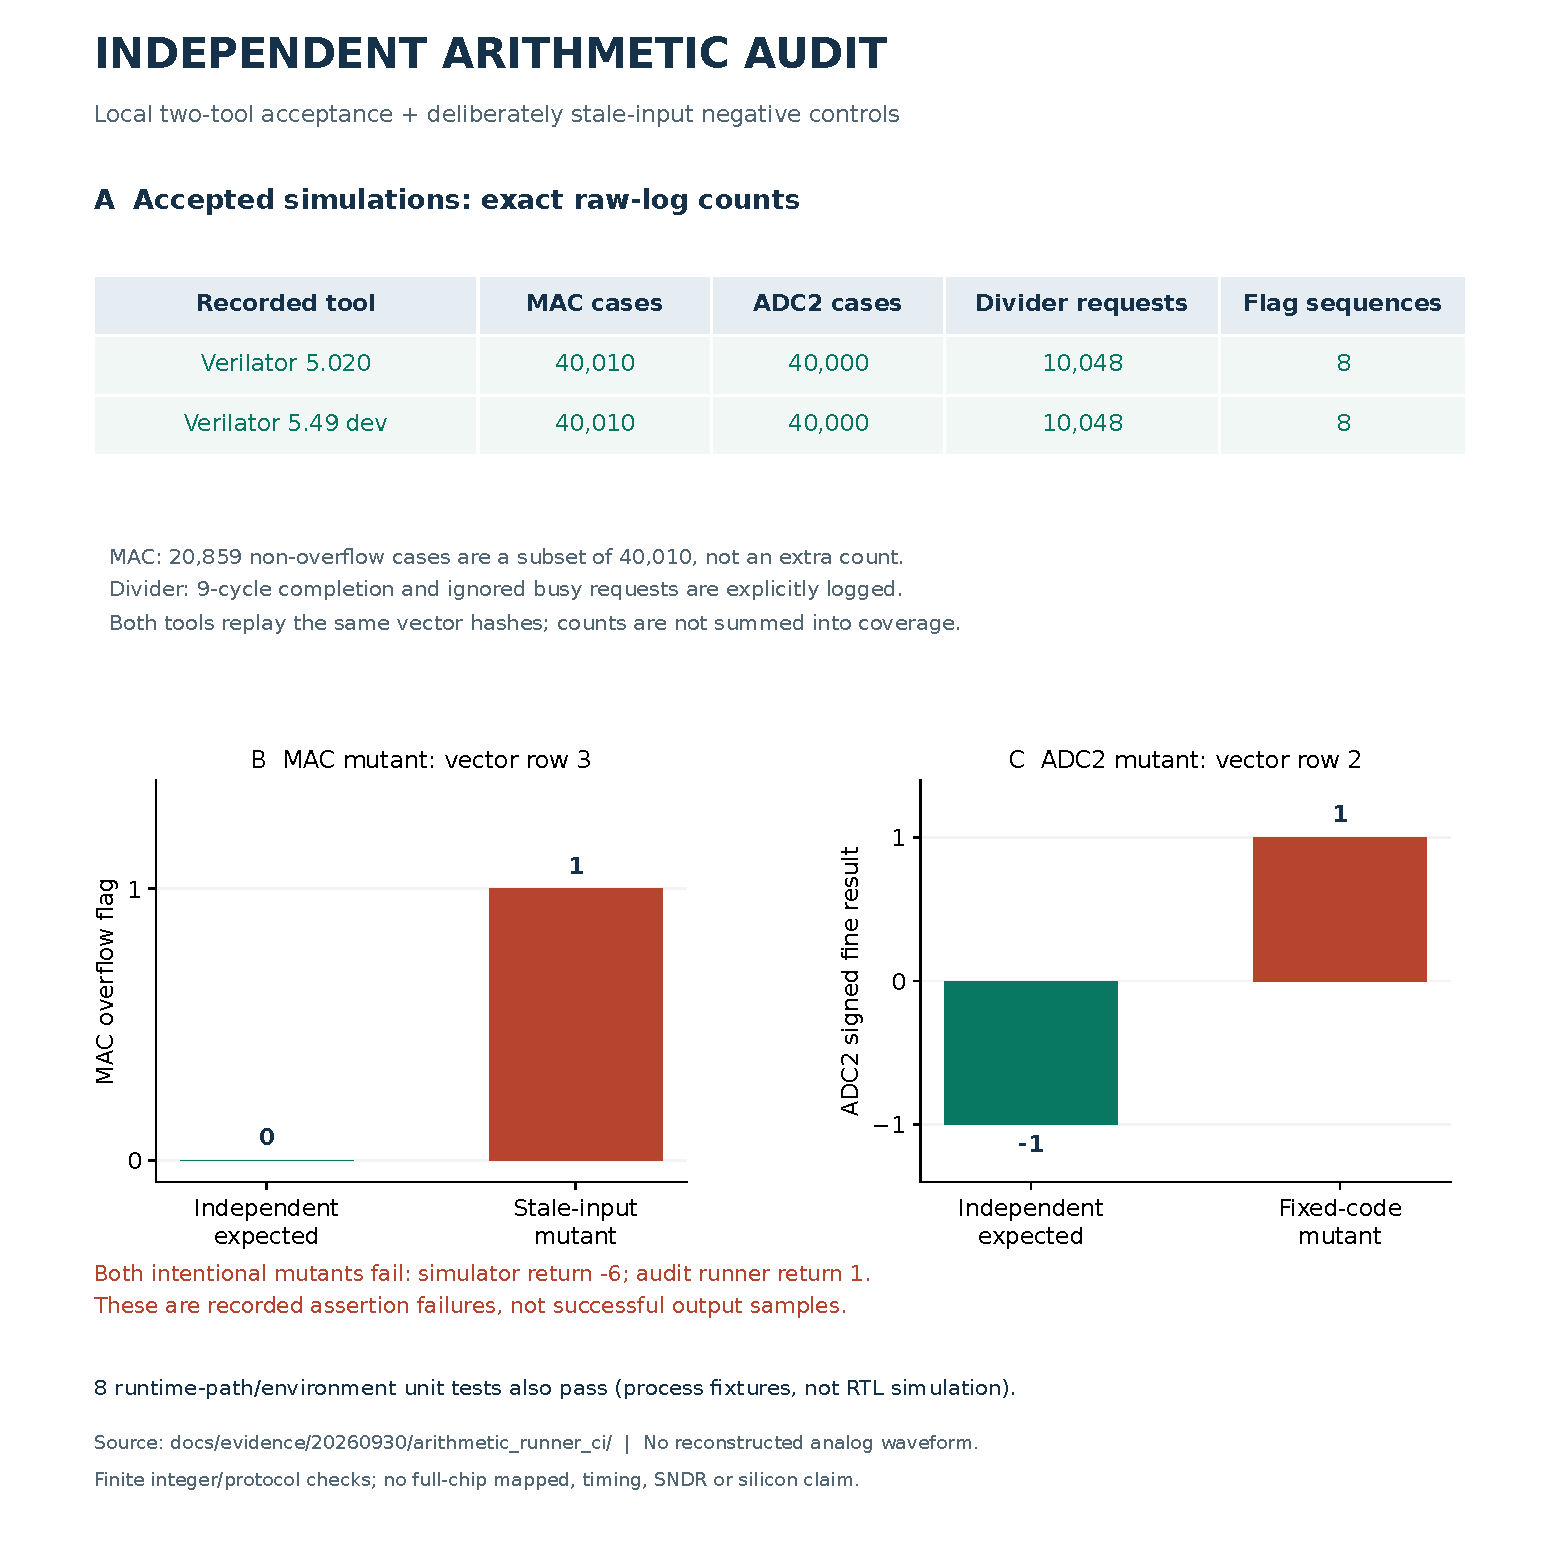
\includegraphics[width=.97\textwidth]{figures/arithmetic_runner_dual_tool.pdf}
\caption{独立算术审计的本地双版本正、负控。上表为各版本原日志的精确计数，20,859 项不溢出 MAC 是 40,010 项的子集。下图只绘制真实失败行：陈旧 MAC 输入使第 3 行溢出标志由期望 0 变为 1；固定 ADC 输入使第 2 行有符号细码由期望 $-1$ 变为 $+1$。两个变异均被独立期望值检出；图不重建波形，也不把负控失败计为正常样本。}
\label{fig:arithmetic-runner-dual-tool}
\end{figure}

\begingroup\raggedright
图\ref{fig:arithmetic-runner-dual-tool} 的脚本为 \code{audit_figures/make_arithmetic_runner_evidence.py}，
来源及数值见 \code{audit_figures/arithmetic_runner_dual_tool.sha256.json}。
两种本地工具重播同一组向量；新 CI 是另一环境复验，三次计数不相加为更大的输入覆盖集合。\par\endgroup

\subsection{重建入口与历史保留}
在报告目录执行 \code{python audit_figures/make_final_regression_evidence.py --schema ci} 可重建四张 PNG/PDF。
脚本校验 CI archive 的 \code{sha256.json}，核对步骤而非仅看 job 总状态，逐字节读取 Git head 中的输入，核对 26 项生产 RTL 集合与 21 份日志，再解析数值和唯一完成标记。
每张同名 \code{audit_figures/final_regression_*.sha256.json} 保存上述来源、测试台行号、图件和脚本摘要；本次 \code{tested_inputs_sha256.json} 摘要为
\par\noindent\code{2e39e58b99e56d04ae7ead3225f1ab44104aaf444219a0190e712d4a8585b774}。

旧 169f 图、PDF、脚本、分节和哈希记录逐字节保留在
\code{history/final_regression_169f_before_ci_0c4a/}，由该目录 \code{archive_manifest.json} 校验。旧 \code{0c4a} CI 的四图、脚本、分节、检查与摘要另存于 \code{history/final_regression_ci_0c4a_before_f028/}；原仓库旧证据没有被覆盖。
图件 \code{31_divider_profiles.png} 仍是另一次 compact 三档生产顶层实跑，每档 438 次输出与延迟检查，不能与本次各 32 笔的连续启动夹具混成一次实验。
本节没有启动新仿真或 EDA，全部图只重建已归档的日志；不提供模拟电路、STA 或硅片性能签核。
